\documentclass[10pt]{article}
\usepackage[margin=0.72in]{geometry}
\usepackage{amsmath,amssymb}
\usepackage{booktabs}
\usepackage{xcolor}
\usepackage{enumitem}
\usepackage{hyperref}
\usepackage{tikz}
\usetikzlibrary{arrows.meta,positioning,fit}

\hypersetup{colorlinks=true,linkcolor=blue,citecolor=blue,urlcolor=blue}
\setlist[itemize]{leftmargin=1.25em,itemsep=2pt,topsep=3pt}
\setlist[enumerate]{leftmargin=1.4em,itemsep=2pt,topsep=3pt}
\setlength{\parindent}{0pt}
\setlength{\parskip}{4pt}

\definecolor{kblue}{RGB}{25,74,120}
\definecolor{kteal}{RGB}{32,130,115}
\definecolor{korange}{RGB}{190,105,35}
\definecolor{kred}{RGB}{155,45,45}
\definecolor{kgray}{RGB}{95,95,95}

\title{\vspace{-1.0cm}\textbf{Kahlus-STF: Leakage-Aware Neural State Transition Forecasting}\\
\large A narrow epilepsy/sleep monitoring concept note for discussion with Robert S. Fisher, MD, PhD}
\author{Aayushya Patel}
\date{\today}

\begin{document}
\maketitle

\vspace{-0.7cm}
\section*{One-sentence claim}
Kahlus-STF is a passive research framework that asks whether a latent state inferred from partial noninvasive EEG/body/sleep observations can forecast future signals, held-out sensors, and probabilistic event-risk windows better than strict baselines under patient-held-out and time-held-out evaluation.

\section*{Why this is worth asking}
Short routine or sleep studies can miss clinically relevant events when the recording does not overlap the event or its surrounding state. Recent evidence supports that prolonged ambulatory EEG can increase diagnostic yield: Li et al. reported diagnostic events in 41\% of prolonged ambulatory video-EEG recordings, with some events captured only on days five to eight \cite{li2024ambulatory}; Hernandez-Ronquillo et al. found 24-hour ambulatory EEG had higher sensitivity for interictal epileptiform discharges/seizures than first or second routine EEG after a first unprovoked seizure \cite{hernandez2023ambulatory}; and Bouma et al. reported low sensitivity for routine EEG in adults after a first unprovoked seizure despite high specificity when epileptiform discharges are present \cite{bouma2016routine}.

This does not mean Kahlus can diagnose epilepsy. It means there is a defensible research target: increase longitudinal evidence capture and forecast future state/risk under rigorous validation, while leaving interpretation to clinicians.

\section*{What Kahlus-STF is not}
\begin{itemize}
  \item Not a diagnostic system, seizure prevention device, treatment engine, medication recommender, or replacement for vEEG/PSG.
  \item Not a stimulation system. The initial scope is passive sensing and retrospective/public-data benchmarking.
  \item Not ``AlphaFold for neurology'' as a current claim. The AlphaFold-level ambition is only a long-term analogy for benchmark discipline, scale, and falsifiability.
\end{itemize}

\section*{Core object}
Let the observed history for person $s$ be
\[
h_t = \{Y_{0:t}, X_{0:t}, Q_{0:t}, M_s\},
\]
where $Y$ is EEG or channel-reduced EEG, $X$ is optional body/sleep context such as PPG/HRV/IMU/sleep stage, $Q$ is signal quality and missingness, and $M_s$ is non-identifying subject/session metadata allowed by the dataset.

Kahlus-STF learns a latent transition state
\[
z_t = f_\theta(h_t)
\]
and evaluates whether it improves calibrated forecasts:
\[
p_\theta(Y_{t+1:t+H}, X_{t+1:t+H}, r_{t+1:t+H} \mid z_t, Q_t),
\]
where $r$ is an event-risk or event-opportunity label only when the dataset provides valid seizure/event annotations.

\begin{figure}[h]
\centering
\resizebox{0.97\linewidth}{!}{%
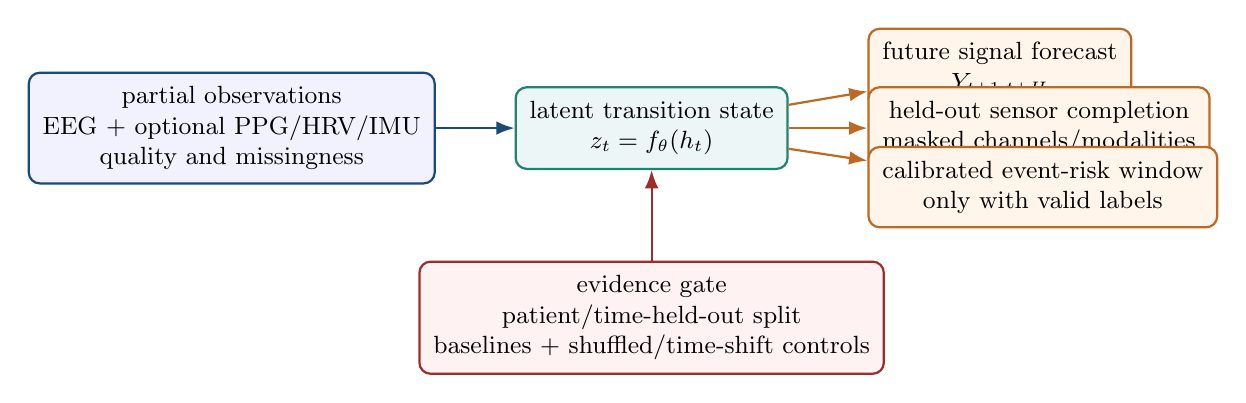
\begin{tikzpicture}[>=Latex,font=\small,node distance=1.1cm]
\tikzstyle{box}=[draw=kblue, thick, rounded corners, fill=blue!5, align=center, inner sep=5pt, minimum height=0.8cm]
\tikzstyle{state}=[draw=kteal, thick, rounded corners, fill=teal!7, align=center, inner sep=5pt, minimum height=0.8cm]
\tikzstyle{head}=[draw=korange, thick, rounded corners, fill=orange!8, align=center, inner sep=5pt, minimum height=0.8cm]
\tikzstyle{gate}=[draw=kred, thick, rounded corners, fill=red!5, align=center, inner sep=5pt, minimum height=0.8cm]

\node[box] (obs) {partial observations\\EEG + optional PPG/HRV/IMU\\quality and missingness};
\node[state, right=1.0cm of obs] (latent) {latent transition state\\$z_t=f_\theta(h_t)$};
\node[head, right=1.0cm of latent, yshift=0.75cm] (forecast) {future signal forecast\\$Y_{t+1:t+H}$};
\node[head, right=1.0cm of latent] (completion) {held-out sensor completion\\masked channels/modalities};
\node[head, right=1.0cm of latent, yshift=-0.75cm] (risk) {calibrated event-risk window\\only with valid labels};
\node[gate, below=1.15cm of latent] (gate) {evidence gate\\patient/time-held-out split\\baselines + shuffled/time-shift controls};

\draw[->, thick, kblue] (obs) -- (latent);
\draw[->, thick, korange] (latent) -- (forecast);
\draw[->, thick, korange] (latent) -- (completion);
\draw[->, thick, korange] (latent) -- (risk);
\draw[->, thick, kred] (gate) -- (latent);
\end{tikzpicture}}
\caption{Kahlus-STF is a passive state-transition benchmark, not a clinical decision system.}
\end{figure}

\section*{Benchmark ladder}
The first implementation should reuse the existing Kahlus v1 discipline: subject/time splits, baseline reporting, shuffled-target controls, and claim gates.

\begin{center}
\begin{tabular}{p{0.24\linewidth}p{0.33\linewidth}p{0.31\linewidth}}
\toprule
Task & Required baselines & Gate failure condition \\
\midrule
Future EEG forecasting & persistence, ridge/AR, TinySSM & model fails to beat autocorrelation baselines \\
Longer-horizon forecasting & persistence, ridge/AR, TinySSM & advantage disappears as horizon increases \\
Held-out channel completion & mean/channel baselines, ridge, TinySSM & completion works only with leakage-prone masks \\
Event-risk forecasting & cycle/time-of-day, diary-frequency, logistic/ridge & no improvement over cyclic or frequency baselines \\
Negative controls & shuffled target, time-shifted labels & control performs close to real task \\
\bottomrule
\end{tabular}
\end{center}

\section*{Why the wearable angle is different}
Wearable seizure detection and forecasting already exist. Systematic reviews show promise, especially for tonic-clonic seizure detection, but also false-alarm, validation, and generalization limits \cite{naganur2022wearables,beniczky2021guideline}. Kahlus should therefore not claim novelty as ``a wearable seizure detector.''

The defensible wearable concept is narrower: a low-burden longitudinal evidence-capture device that increases the chance of observing relevant sleep/neural/body transitions and then runs a claim-gated forecasting benchmark. A future v0 device could use limited EEG plus PPG/HRV and IMU, but the first sprint should remain retrospective and public-data based.

\section*{Math stop note}
Before any new model is added, the implementation should answer four questions in writing:
\begin{enumerate}
  \item What object is modeled? A latent transition state $z_t$ inferred from allowed history.
  \item What must it beat? Persistence, ridge/AR, TinySSM, cycle/time-of-day, and negative controls.
  \item What leakage could fake success? Adjacent windows, subject identity, overlapping events, post-event labels, duplicated segments, and non-held-out calibration.
  \item What would falsify it? Baselines dominate, shuffled/time-shift controls perform similarly, calibration fails, or patient-held-out performance collapses.
\end{enumerate}

\section*{Questions for Dr. Fisher}
\begin{enumerate}
  \item Is passive longitudinal state-transition forecasting a clinically meaningful framing, or is event detection/counting the only defensible near-term target?
  \item Which public or collaborative epilepsy datasets would be appropriate for patient-held-out, time-held-out benchmarking?
  \item Which metrics would matter most to an epilepsy clinician: false alarms per day, time in warning, event sensitivity, calibration, seizure burden estimation, or review-time reduction?
  \item Is the wearable concept most useful for missed nocturnal events, focal seizures, seizure burden tracking, or scheduling higher-yield clinical EEG?
\end{enumerate}

\section*{Claim boundary}
Allowed language: research benchmark, passive longitudinal monitoring support, signal-quality flags, future signal forecasting, held-out sensor completion, calibrated event-risk windows, clinician-reviewed evidence.

Blocked language: diagnoses epilepsy, predicts seizures clinically, prevents seizures, adjusts medication, replaces EEG/vEEG/PSG, treats epilepsy, or proves a neurology foundation model.

\begin{thebibliography}{9}
\bibitem{li2024ambulatory}
M. C. Li et al.,
\href{https://consensus.app/papers/details/9ca353f770245b4d82aacc65aae8e37b/?utm_source=unknown}{Diagnostic utility of prolonged ambulatory video-electroencephalography monitoring},
\emph{Epilepsy \& Behavior}, 2024.

\bibitem{hernandez2023ambulatory}
L. Hernandez-Ronquillo et al.,
\href{https://consensus.app/papers/details/3eb9fac24173596da8c7ae3d6d60e879/?utm_source=unknown}{Diagnostic Accuracy of Ambulatory EEG vs Routine EEG in Patients With First Single Unprovoked Seizure},
\emph{Neurology: Clinical Practice}, 2023.

\bibitem{bouma2016routine}
H. Bouma et al.,
\href{https://consensus.app/papers/details/e93de1b6e0755abe8176fef442024c32/?utm_source=unknown}{The diagnostic accuracy of routine electroencephalography after a first unprovoked seizure},
\emph{European Journal of Neurology}, 2016.

\bibitem{naganur2022wearables}
V. Naganur et al.,
\href{https://consensus.app/papers/details/88c1d0d7ea71587e9248a9cc3d9a5041/?utm_source=unknown}{Automated seizure detection with noninvasive wearable devices: A systematic review and meta-analysis},
\emph{Epilepsia}, 2022.

\bibitem{beniczky2021guideline}
S. Beniczky et al.,
\href{https://consensus.app/papers/details/f4e568f079ca50a9b96a4d0313e3f410/?utm_source=unknown}{Automated seizure detection using wearable devices: A clinical practice guideline of the International League Against Epilepsy and the International Federation of Clinical Neurophysiology},
\emph{Epilepsia}, 2021.

\bibitem{carmo2024forecast}
A. S. Carmo et al.,
\href{https://consensus.app/papers/details/bd024f0e465d5f1e9b70ded08334df4b/?utm_source=unknown}{Automated algorithms for seizure forecast: a systematic review and meta-analysis},
\emph{Journal of Neurology}, 2024.

\bibitem{shafiezadeh2024crosspatient}
S. Shafiezadeh et al.,
\href{https://consensus.app/papers/details/9a161ced16705127bce6b5fd257f33ce/?utm_source=unknown}{A systematic review of cross-patient approaches for EEG epileptic seizure prediction},
\emph{Journal of Neural Engineering}, 2024.
\end{thebibliography}

\end{document}
